%! TEX root = ../dsa-review.tex

For a string $T$, substring of $T$ is denoted by $T[i,j]$ where $0 \leq i \leq j < M$.

\begin{description}
  \item[Prefix] Substring from $0$ to $i$ where $i < M$
  \item[Suffix] Substring from $i$ to $M - 1$ where $i \geq 0$
\end{description}

\section{Brute-force String Pattern Matching}

Suppose we want to check if a string $P$ (stands for "pattern") is a substring of a longer string $T$.
If you are lazy, you can use the following brute-force pattern-matching algorithm.

\begin{minted}{python}
  def bruteForceMatch(T, P):  # P is the "pattern" string we wish to find in T
      n, m = len(T), len(P)
      for i in range(n - m):
          j = 0
          while j < m and T[i + j] == P[j]:
              j += 1
          if j == m:
              return i

      return -1
\end{minted}

\noindent The algorithm goes through $T$ and checks compares characters of $P$ until we reach the end $P$, returning the earliest match.
The algorithm is highly inefficient, taking $O(nm)$ time in the worst case scenario.

\begin{center}
  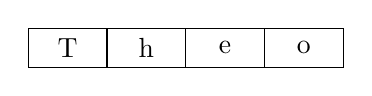
\begin{tikzpicture}
    \node [draw, minimum width=1cm, minimum height=0.5cm] at (0, 1) {T};
    \node [draw, minimum width=1cm, minimum height=0.5cm] at (1, 1) {h};
    \node [draw, minimum width=1cm, minimum height=0.5cm] at (2, 1) {e};
    \node [draw, minimum width=1cm, minimum height=0.5cm] at (3, 1) {o};
  \end{tikzpicture}

  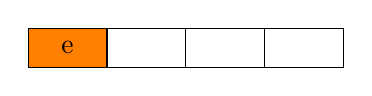
\begin{tikzpicture}
    \node [draw, minimum width=1cm, minimum height=0.5cm, fill=orange] at (0, 1) {e};
    \node [draw, minimum width=1cm, minimum height=0.5cm] at (1, 1) {};
    \node [draw, minimum width=1cm, minimum height=0.5cm] at (2, 1) {};
    \node [draw, minimum width=1cm, minimum height=0.5cm] at (3, 1) {};
  \end{tikzpicture}

  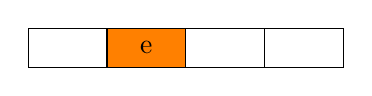
\begin{tikzpicture}
    \node [draw, minimum width=1cm, minimum height=0.5cm] at (0, 1) {};
    \node [draw, minimum width=1cm, minimum height=0.5cm, fill=orange] at (1, 1) {e};
    \node [draw, minimum width=1cm, minimum height=0.5cm] at (2, 1) {};
    \node [draw, minimum width=1cm, minimum height=0.5cm] at (3, 1) {};
  \end{tikzpicture}

  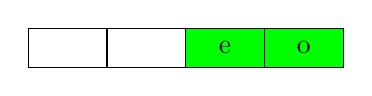
\begin{tikzpicture}
    \node [draw, minimum width=1cm, minimum height=0.5cm] at (0, 1) {};
    \node [draw, minimum width=1cm, minimum height=0.5cm] at (1, 1) {};
    \node [draw, minimum width=1cm, minimum height=0.5cm, fill=green] at (2, 1) {e};
    \node [draw, minimum width=1cm, minimum height=0.5cm, fill=green] at (3, 1) {o};
  \end{tikzpicture}
\end{center}

\section{KMP Algorithm}

Knuth-Morris-Pratt algorithm is an efficient pattern matching algorithm with $O(n + m)$ time complexity.

\noindent It uses the pre-computed \textsc{LPS} (Longest Proper Prefix, where proper prefix is a prefix of $T$ that does not include $T$ itself) array.
The name \textsc{LPS} is slightly misleading, as what \textsc{Failure} function is actually calculating is \textbf{the length of the longest matching prefix \& suffix for each substring}.

\begin{minted}{python}
  def failure(pattern):
      m = len(pattern)
      lps = [0] * m
      j = 0
      for i in range(1, m):
          while j > 0 and pattern[i] != pattern[j]:
              j = lps[j - 1]
          if pattern[i] == pattern[j]:
              j += 1
          lps[i] = j

      return lps
\end{minted}

\noindent For example, for the string \textsc{"ababcab"}, the \textsc{Failure} function produces the following result.

\begin{align*}
  &\mathrm{lps} = \mathrm{failure}(``ababcab'') \\
  &\mathrm{lps}[0] = 0 & (``a'') \\
  &\mathrm{lps}[1] = 0 & (``ab") \\
  &\mathrm{lps}[2] = 1 & (``\mathbf{\overline{a}}b\mathbf{\overline{a}}") \\
  &\mathrm{lps}[3] = 2 & (``\mathbf{\overline{ab}}\ \mathbf{\overline{ab}}") \\
  &\mathrm{lps}[4] = 0 & (``ababc") \\
  &\mathrm{lps}[5] = 1 & (``\mathbf{\overline{a}}babc\mathbf{\overline{a}}") \\
  &\mathrm{lps}[6] = 2 & (``\mathbf{\overline{ab}}abc\mathbf{\overline{ab}}")
\end{align*}

\noindent The \textsc{KMP} driver function uses the \textsc{LPS} array to find the earliest index where the pattern is found.

\begin{minted}{python}
  def kmp(T, pattern):
      n, m = len(T), len(pattern)
      lps = failure(T, pattern)
      i, j = 0, 0
      while i < n:
          if T[i] == pattern[j]:
              if j == m - 1:
                  return i - j
              else:
                  i += 1
                  j += 1
          elif j > 0:
              j = lps[j - 1]
          else:
              i += 1
      return -1
\end{minted}

\begin{center}
  \colorbox{white}{\makebox(9,9){\textcolor{black}{a}}}
  \colorbox{white}{\makebox(9,9){\textcolor{black}{b}}}
  \colorbox{white}{\makebox(9,9){\textcolor{black}{a}}}
  \colorbox{white}{\makebox(9,9){\textcolor{black}{b}}}
  \colorbox{white}{\makebox(9,9){\textcolor{black}{c}}}
  \colorbox{white}{\makebox(9,9){\textcolor{black}{a}}}
  \colorbox{white}{\makebox(9,9){\textcolor{black}{a}}}
  \colorbox{white}{\makebox(9,9){\textcolor{black}{b}}}
  \colorbox{white}{\makebox(9,9){\textcolor{black}{a}}}
  \colorbox{white}{\makebox(9,9){\textcolor{black}{c}}}
  \colorbox{white}{\makebox(9,9){\textcolor{black}{c}}}
  \colorbox{white}{\makebox(9,9){\textcolor{black}{a}}}
  \colorbox{white}{\makebox(9,9){\textcolor{black}{b}}}
  \colorbox{white}{\makebox(9,9){\textcolor{black}{a}}}
  \colorbox{white}{\makebox(9,9){\textcolor{black}{b}}}
  \colorbox{white}{\makebox(9,9){\textcolor{black}{c}}}
  \colorbox{white}{\makebox(9,9){\textcolor{black}{a}}}
  \colorbox{white}{\makebox(9,9){\textcolor{black}{b}}}
  \\
  \colorbox{green}{\makebox(9,9){\textcolor{black}{a}}}
  \colorbox{green}{\makebox(9,9){\textcolor{black}{b}}}
  \colorbox{green}{\makebox(9,9){\textcolor{black}{a}}}
  \colorbox{green}{\makebox(9,9){\textcolor{black}{b}}}
  \colorbox{green}{\makebox(9,9){\textcolor{black}{c}}}
  \colorbox{green}{\makebox(9,9){\textcolor{black}{a}}}
  \colorbox{orange}{\makebox(9,9){\textcolor{black}{b}}}
  \colorbox{white}{\makebox(9,9){\textcolor{black}{}}}
  \colorbox{white}{\makebox(9,9){\textcolor{black}{}}}
  \colorbox{white}{\makebox(9,9){\textcolor{black}{}}}
  \colorbox{white}{\makebox(9,9){\textcolor{black}{}}}
  \colorbox{white}{\makebox(9,9){\textcolor{black}{}}}
  \colorbox{white}{\makebox(9,9){\textcolor{black}{}}}
  \colorbox{white}{\makebox(9,9){\textcolor{black}{}}}
  \colorbox{white}{\makebox(9,9){\textcolor{black}{}}}
  \colorbox{white}{\makebox(9,9){\textcolor{black}{}}}
  \colorbox{white}{\makebox(9,9){\textcolor{black}{}}}
  \colorbox{white}{\makebox(9,9){\textcolor{black}{}}}
  \\
  Since the length of longest prefix/suffix is 1 (\textsc{``a''}), start matching at index 1.
  \\
  \colorbox{gray}{\makebox(9,9){\textcolor{black}{}}}
  \colorbox{gray}{\makebox(9,9){\textcolor{black}{}}}
  \colorbox{gray}{\makebox(9,9){\textcolor{black}{}}}
  \colorbox{gray}{\makebox(9,9){\textcolor{black}{}}}
  \colorbox{gray}{\makebox(9,9){\textcolor{black}{}}}
  \colorbox{cyan}{\makebox(9,9){\textcolor{black}{a}}}
  \colorbox{orange}{\makebox(9,9){\textcolor{black}{b}}}
  \colorbox{white}{\makebox(9,9){\textcolor{black}{}}}
  \colorbox{white}{\makebox(9,9){\textcolor{black}{}}}
  \colorbox{white}{\makebox(9,9){\textcolor{black}{}}}
  \colorbox{white}{\makebox(9,9){\textcolor{black}{}}}
  \colorbox{white}{\makebox(9,9){\textcolor{black}{}}}
  \colorbox{white}{\makebox(9,9){\textcolor{black}{}}}
  \colorbox{white}{\makebox(9,9){\textcolor{black}{}}}
  \colorbox{white}{\makebox(9,9){\textcolor{black}{}}}
  \colorbox{white}{\makebox(9,9){\textcolor{black}{}}}
  \colorbox{white}{\makebox(9,9){\textcolor{black}{}}}
  \colorbox{white}{\makebox(9,9){\textcolor{black}{}}}
  \\
  Since the length of longest prefix/suffix is 0, start matching at index 0.
  \\
  \colorbox{gray}{\makebox(9,9){\textcolor{black}{}}}
  \colorbox{gray}{\makebox(9,9){\textcolor{black}{}}}
  \colorbox{gray}{\makebox(9,9){\textcolor{black}{}}}
  \colorbox{gray}{\makebox(9,9){\textcolor{black}{}}}
  \colorbox{gray}{\makebox(9,9){\textcolor{black}{}}}
  \colorbox{gray}{\makebox(9,9){\textcolor{black}{}}}
  \colorbox{green}{\makebox(9,9){\textcolor{black}{a}}}
  \colorbox{green}{\makebox(9,9){\textcolor{black}{b}}}
  \colorbox{green}{\makebox(9,9){\textcolor{black}{a}}}
  \colorbox{orange}{\makebox(9,9){\textcolor{black}{b}}}
  \colorbox{white}{\makebox(9,9){\textcolor{black}{}}}
  \colorbox{white}{\makebox(9,9){\textcolor{black}{}}}
  \colorbox{white}{\makebox(9,9){\textcolor{black}{}}}
  \colorbox{white}{\makebox(9,9){\textcolor{black}{}}}
  \colorbox{white}{\makebox(9,9){\textcolor{black}{}}}
  \colorbox{white}{\makebox(9,9){\textcolor{black}{}}}
  \colorbox{white}{\makebox(9,9){\textcolor{black}{}}}
  \colorbox{white}{\makebox(9,9){\textcolor{black}{}}}
  \\
  Since the length of longest prefix/suffix is 1 (\textsc{``a''}), start matching at index 1.
  \\
  \colorbox{gray}{\makebox(9,9){\textcolor{black}{}}}
  \colorbox{gray}{\makebox(9,9){\textcolor{black}{}}}
  \colorbox{gray}{\makebox(9,9){\textcolor{black}{}}}
  \colorbox{gray}{\makebox(9,9){\textcolor{black}{}}}
  \colorbox{gray}{\makebox(9,9){\textcolor{black}{}}}
  \colorbox{gray}{\makebox(9,9){\textcolor{black}{}}}
  \colorbox{gray}{\makebox(9,9){\textcolor{black}{}}}
  \colorbox{gray}{\makebox(9,9){\textcolor{black}{}}}
  \colorbox{cyan}{\makebox(9,9){\textcolor{black}{a}}}
  \colorbox{orange}{\makebox(9,9){\textcolor{black}{b}}}
  \colorbox{white}{\makebox(9,9){\textcolor{black}{}}}
  \colorbox{white}{\makebox(9,9){\textcolor{black}{}}}
  \colorbox{white}{\makebox(9,9){\textcolor{black}{}}}
  \colorbox{white}{\makebox(9,9){\textcolor{black}{}}}
  \colorbox{white}{\makebox(9,9){\textcolor{black}{}}}
  \colorbox{white}{\makebox(9,9){\textcolor{black}{}}}
  \colorbox{white}{\makebox(9,9){\textcolor{black}{}}}
  \colorbox{white}{\makebox(9,9){\textcolor{black}{}}}
  \\
  Since the length of longest prefix/suffix is 0, start matching at index 0.
  \\
  \colorbox{gray}{\makebox(9,9){\textcolor{black}{}}}
  \colorbox{gray}{\makebox(9,9){\textcolor{black}{}}}
  \colorbox{gray}{\makebox(9,9){\textcolor{black}{}}}
  \colorbox{gray}{\makebox(9,9){\textcolor{black}{}}}
  \colorbox{gray}{\makebox(9,9){\textcolor{black}{}}}
  \colorbox{gray}{\makebox(9,9){\textcolor{black}{}}}
  \colorbox{gray}{\makebox(9,9){\textcolor{black}{}}}
  \colorbox{gray}{\makebox(9,9){\textcolor{black}{}}}
  \colorbox{gray}{\makebox(9,9){\textcolor{black}{}}}
  \colorbox{orange}{\makebox(9,9){\textcolor{black}{a}}}
  \colorbox{white}{\makebox(9,9){\textcolor{black}{}}}
  \colorbox{white}{\makebox(9,9){\textcolor{black}{}}}
  \colorbox{white}{\makebox(9,9){\textcolor{black}{}}}
  \colorbox{white}{\makebox(9,9){\textcolor{black}{}}}
  \colorbox{white}{\makebox(9,9){\textcolor{black}{}}}
  \colorbox{white}{\makebox(9,9){\textcolor{black}{}}}
  \colorbox{white}{\makebox(9,9){\textcolor{black}{}}}
  \colorbox{white}{\makebox(9,9){\textcolor{black}{}}}
  \\
  Since the length of longest prefix/suffix is 0, start matching at index 0.
  \\
  \colorbox{gray}{\makebox(9,9){\textcolor{black}{}}}
  \colorbox{gray}{\makebox(9,9){\textcolor{black}{}}}
  \colorbox{gray}{\makebox(9,9){\textcolor{black}{}}}
  \colorbox{gray}{\makebox(9,9){\textcolor{black}{}}}
  \colorbox{gray}{\makebox(9,9){\textcolor{black}{}}}
  \colorbox{gray}{\makebox(9,9){\textcolor{black}{}}}
  \colorbox{gray}{\makebox(9,9){\textcolor{black}{}}}
  \colorbox{gray}{\makebox(9,9){\textcolor{black}{}}}
  \colorbox{gray}{\makebox(9,9){\textcolor{black}{}}}
  \colorbox{gray}{\makebox(9,9){\textcolor{black}{}}}
  \colorbox{orange}{\makebox(9,9){\textcolor{black}{a}}}
  \colorbox{white}{\makebox(9,9){\textcolor{black}{}}}
  \colorbox{white}{\makebox(9,9){\textcolor{black}{}}}
  \colorbox{white}{\makebox(9,9){\textcolor{black}{}}}
  \colorbox{white}{\makebox(9,9){\textcolor{black}{}}}
  \colorbox{white}{\makebox(9,9){\textcolor{black}{}}}
  \colorbox{white}{\makebox(9,9){\textcolor{black}{}}}
  \colorbox{white}{\makebox(9,9){\textcolor{black}{}}}
  \\
  Since the length of longest prefix/suffix is 0, start matching at index 0.
  \\
  \colorbox{gray}{\makebox(9,9){\textcolor{black}{}}}
  \colorbox{gray}{\makebox(9,9){\textcolor{black}{}}}
  \colorbox{gray}{\makebox(9,9){\textcolor{black}{}}}
  \colorbox{gray}{\makebox(9,9){\textcolor{black}{}}}
  \colorbox{gray}{\makebox(9,9){\textcolor{black}{}}}
  \colorbox{gray}{\makebox(9,9){\textcolor{black}{}}}
  \colorbox{gray}{\makebox(9,9){\textcolor{black}{}}}
  \colorbox{gray}{\makebox(9,9){\textcolor{black}{}}}
  \colorbox{gray}{\makebox(9,9){\textcolor{black}{}}}
  \colorbox{gray}{\makebox(9,9){\textcolor{black}{}}}
  \colorbox{gray}{\makebox(9,9){\textcolor{black}{}}}
  \colorbox{green}{\makebox(9,9){\textcolor{black}{a}}}
  \colorbox{green}{\makebox(9,9){\textcolor{black}{b}}}
  \colorbox{green}{\makebox(9,9){\textcolor{black}{a}}}
  \colorbox{green}{\makebox(9,9){\textcolor{black}{b}}}
  \colorbox{green}{\makebox(9,9){\textcolor{black}{a}}}
  \colorbox{green}{\makebox(9,9){\textcolor{black}{a}}}
  \colorbox{green}{\makebox(9,9){\textcolor{black}{b}}}
\end{center}

\noindent Okay, kind of a bad example, here is a simpler example with $T = abacaabaccabacab$ and $P = abacab$.

\begin{align*}
  &\mathrm{lps} = \mathrm{failure}(``abacab'') \\
  &\mathrm{lps}[0] = 0 & (``a'') \\
  &\mathrm{lps}[1] = 0 & (``ab") \\
  &\mathrm{lps}[2] = 1 & (``\mathbf{\overline{a}}b\mathbf{\overline{a}}") \\
  &\mathrm{lps}[3] = 0 & (``abac") \\
  &\mathrm{lps}[4] = 1 & (``\mathbf{\overline{a}}bac\mathbf{\overline{a}}") \\
  &\mathrm{lps}[5] = 2 & (``\mathbf{\overline{ab}}ac\mathbf{\overline{ab}}") \\
\end{align*}

\begin{center}
  \colorbox{white}{\makebox(9,9){\textcolor{black}{a}}}
  \colorbox{white}{\makebox(9,9){\textcolor{black}{b}}}
  \colorbox{white}{\makebox(9,9){\textcolor{black}{a}}}
  \colorbox{white}{\makebox(9,9){\textcolor{black}{c}}}
  \colorbox{white}{\makebox(9,9){\textcolor{black}{a}}}
  \colorbox{white}{\makebox(9,9){\textcolor{black}{a}}}
  \colorbox{white}{\makebox(9,9){\textcolor{black}{b}}}
  \colorbox{white}{\makebox(9,9){\textcolor{black}{a}}}
  \colorbox{white}{\makebox(9,9){\textcolor{black}{c}}}
  \colorbox{white}{\makebox(9,9){\textcolor{black}{c}}}
  \colorbox{white}{\makebox(9,9){\textcolor{black}{a}}}
  \colorbox{white}{\makebox(9,9){\textcolor{black}{b}}}
  \colorbox{white}{\makebox(9,9){\textcolor{black}{a}}}
  \colorbox{white}{\makebox(9,9){\textcolor{black}{c}}}
  \colorbox{white}{\makebox(9,9){\textcolor{black}{a}}}
  \colorbox{white}{\makebox(9,9){\textcolor{black}{b}}}
  \\
  \colorbox{green}{\makebox(9,9){\textcolor{black}{a}}}
  \colorbox{green}{\makebox(9,9){\textcolor{black}{b}}}
  \colorbox{green}{\makebox(9,9){\textcolor{black}{a}}}
  \colorbox{green}{\makebox(9,9){\textcolor{black}{c}}}
  \colorbox{green}{\makebox(9,9){\textcolor{black}{a}}}
  \colorbox{orange}{\makebox(9,9){\textcolor{black}{b}}}
  \colorbox{white}{\makebox(9,9){\textcolor{black}{}}}
  \colorbox{white}{\makebox(9,9){\textcolor{black}{}}}
  \colorbox{white}{\makebox(9,9){\textcolor{black}{}}}
  \colorbox{white}{\makebox(9,9){\textcolor{black}{}}}
  \colorbox{white}{\makebox(9,9){\textcolor{black}{}}}
  \colorbox{white}{\makebox(9,9){\textcolor{black}{}}}
  \colorbox{white}{\makebox(9,9){\textcolor{black}{}}}
  \colorbox{white}{\makebox(9,9){\textcolor{black}{}}}
  \colorbox{white}{\makebox(9,9){\textcolor{black}{}}}
  \colorbox{white}{\makebox(9,9){\textcolor{black}{}}}
  \\
  Since the length of longest prefix/suffix is 1 (\textsc{``a''}), start matching at index 1.
  \\
  \colorbox{gray}{\makebox(9,9){\textcolor{black}{}}}
  \colorbox{gray}{\makebox(9,9){\textcolor{black}{}}}
  \colorbox{gray}{\makebox(9,9){\textcolor{black}{}}}
  \colorbox{gray}{\makebox(9,9){\textcolor{black}{}}}
  \colorbox{cyan}{\makebox(9,9){\textcolor{black}{a}}}
  \colorbox{orange}{\makebox(9,9){\textcolor{black}{b}}}
  \colorbox{white}{\makebox(9,9){\textcolor{black}{}}}
  \colorbox{white}{\makebox(9,9){\textcolor{black}{}}}
  \colorbox{white}{\makebox(9,9){\textcolor{black}{}}}
  \colorbox{white}{\makebox(9,9){\textcolor{black}{}}}
  \colorbox{white}{\makebox(9,9){\textcolor{black}{}}}
  \colorbox{white}{\makebox(9,9){\textcolor{black}{}}}
  \colorbox{white}{\makebox(9,9){\textcolor{black}{}}}
  \colorbox{white}{\makebox(9,9){\textcolor{black}{}}}
  \colorbox{white}{\makebox(9,9){\textcolor{black}{}}}
  \colorbox{white}{\makebox(9,9){\textcolor{black}{}}}
  \\
  Since the length of longest prefix/suffix is 0, start matching at index 0.
  \\
  \colorbox{gray}{\makebox(9,9){\textcolor{black}{}}}
  \colorbox{gray}{\makebox(9,9){\textcolor{black}{}}}
  \colorbox{gray}{\makebox(9,9){\textcolor{black}{}}}
  \colorbox{gray}{\makebox(9,9){\textcolor{black}{}}}
  \colorbox{gray}{\makebox(9,9){\textcolor{black}{}}}
  \colorbox{green}{\makebox(9,9){\textcolor{black}{a}}}
  \colorbox{green}{\makebox(9,9){\textcolor{black}{b}}}
  \colorbox{green}{\makebox(9,9){\textcolor{black}{a}}}
  \colorbox{green}{\makebox(9,9){\textcolor{black}{c}}}
  \colorbox{orange}{\makebox(9,9){\textcolor{black}{a}}}
  \colorbox{white}{\makebox(9,9){\textcolor{black}{}}}
  \colorbox{white}{\makebox(9,9){\textcolor{black}{}}}
  \colorbox{white}{\makebox(9,9){\textcolor{black}{}}}
  \colorbox{white}{\makebox(9,9){\textcolor{black}{}}}
  \colorbox{white}{\makebox(9,9){\textcolor{black}{}}}
  \colorbox{white}{\makebox(9,9){\textcolor{black}{}}}
  \\
  Since the length of longest prefix/suffix is 0, start matching at index 0.
  \\
  \colorbox{gray}{\makebox(9,9){\textcolor{black}{}}}
  \colorbox{gray}{\makebox(9,9){\textcolor{black}{}}}
  \colorbox{gray}{\makebox(9,9){\textcolor{black}{}}}
  \colorbox{gray}{\makebox(9,9){\textcolor{black}{}}}
  \colorbox{gray}{\makebox(9,9){\textcolor{black}{}}}
  \colorbox{gray}{\makebox(9,9){\textcolor{black}{}}}
  \colorbox{gray}{\makebox(9,9){\textcolor{black}{}}}
  \colorbox{gray}{\makebox(9,9){\textcolor{black}{}}}
  \colorbox{gray}{\makebox(9,9){\textcolor{black}{}}}
  \colorbox{orange}{\makebox(9,9){\textcolor{black}{a}}}
  \colorbox{white}{\makebox(9,9){\textcolor{black}{}}}
  \colorbox{white}{\makebox(9,9){\textcolor{black}{}}}
  \colorbox{white}{\makebox(9,9){\textcolor{black}{}}}
  \colorbox{white}{\makebox(9,9){\textcolor{black}{}}}
  \colorbox{white}{\makebox(9,9){\textcolor{black}{}}}
  \colorbox{white}{\makebox(9,9){\textcolor{black}{}}}
  \\
  Since the length of longest prefix/suffix is 0, start matching at index 0.
  \\
  \colorbox{gray}{\makebox(9,9){\textcolor{black}{}}}
  \colorbox{gray}{\makebox(9,9){\textcolor{black}{}}}
  \colorbox{gray}{\makebox(9,9){\textcolor{black}{}}}
  \colorbox{gray}{\makebox(9,9){\textcolor{black}{}}}
  \colorbox{gray}{\makebox(9,9){\textcolor{black}{}}}
  \colorbox{gray}{\makebox(9,9){\textcolor{black}{}}}
  \colorbox{gray}{\makebox(9,9){\textcolor{black}{}}}
  \colorbox{gray}{\makebox(9,9){\textcolor{black}{}}}
  \colorbox{gray}{\makebox(9,9){\textcolor{black}{}}}
  \colorbox{gray}{\makebox(9,9){\textcolor{black}{}}}
  \colorbox{green}{\makebox(9,9){\textcolor{black}{a}}}
  \colorbox{green}{\makebox(9,9){\textcolor{black}{b}}}
  \colorbox{green}{\makebox(9,9){\textcolor{black}{a}}}
  \colorbox{green}{\makebox(9,9){\textcolor{black}{c}}}
  \colorbox{green}{\makebox(9,9){\textcolor{black}{a}}}
  \colorbox{green}{\makebox(9,9){\textcolor{black}{b}}}
\end{center}

\noindent Okay, that was also not a good example, but hope you get the gist; when a failure in matcing occurs, KMP algorithm skips searching the part where the prefix and suffix is known to match.

\section{Trie}

A trie, or a prefix tree is a specialized search tree for storing characters of strings.

\begin{center}
  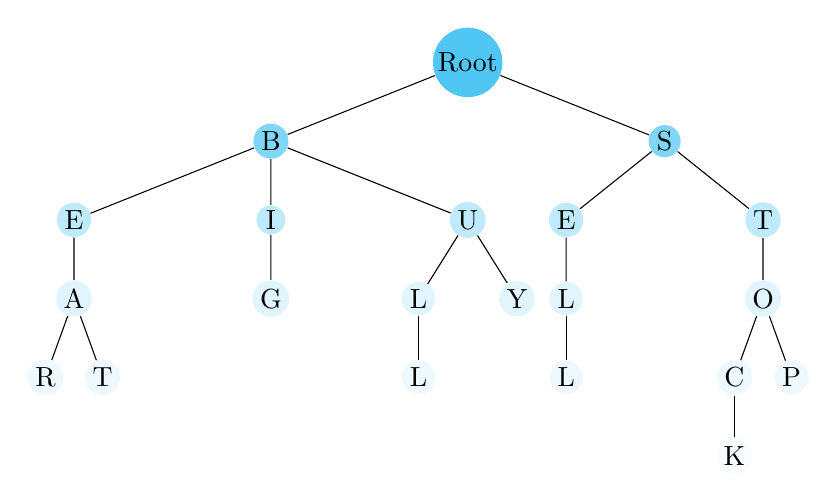
\begin{tikzpicture}
    [
    level distance=10mm,
    every node/.style={fill=cyan!69,circle,inner sep=1pt},
    level 1/.style={sibling distance=50mm,nodes={fill=cyan!50}},
    level 2/.style={sibling distance=25mm,nodes={fill=cyan!25}},
    level 3/.style={sibling distance=12.5mm,nodes={fill=cyan!12}},
    level 4/.style={sibling distance=7.25mm,nodes={fill=cyan!7}},
    level 5/.style={sibling distance=3.625mm,nodes={fill=cyan!3}},
    ]
    \node {Root}
    child {node {B}
      child {node {E}
        child {node {A}
          child {node {R} }
          child {node {T} }
        }
      }
      child {node {I}
        child {node {G}}
      }
      child {node {U}
        child {node {L}
          child {node {L} }
        }
        child {node {Y} }
      }
    }
    child {node {S}
      child {node {E}
        child {node {L}
          child {node {L} }
        }
      }
      child {node {T}
        child {node {O}
          child {node {C}
            child {node {K} }
          }
          child {node {P} }
        }
      }
    };
  \end{tikzpicture}
  \\
  Trie with the following words: { BEAR, BEAT, BIG, BULL, BUY, SELL, STOCK, STOP }
\end{center}

\noindent Following is the implementation of Trie in Python and the basic visualization method.

\begin{minted}{python}
  class TrieNode:
      def __init__(self):
          self.children = {}
          self.end = False
          self.freq = 0


  class Trie:
      def __init__(self):
          self.root = TrieNode()

      def insert(self, word):
          """
          Inserts the given string in the Trie
          :param word: string to be inserted
          """
          node = self.root
          for c in word:
              if c not in node.children:
                  node.children[c] = TrieNode()
              node = node.children[c]
              node.freq += 1
          node.end = True

      def visualize(self):
          def dfs(node, prefix="", indent=""):
              for char, child in sorted(node.children.items()):
                  marker = "*" if child.end else ""
                  print(f"{indent}{char}{marker}")
                  dfs(child, prefix + char, indent + " ")

          print("ROOT")
          dfs(self.root)
\end{minted}

\noindent The visualization, unfortunately, is not in the traditional top-down tree form, as the implementation of such visualization is vastly more complicated.
Instead, the Trie above would be shown as the following:

\begin{verbatim}
    trie = Trie()
    trie.insert("BEAR")
    trie.insert("BEAT")
    trie.insert("BIG")
    trie.insert("BULL")
    trie.insert("BUY")
    trie.insert("SELL")
    trie.insert("STOCK")
    trie.insert("STOP")
    trie.visualize()

    ...
    B
     E
      A
       R*
       T*
     I
      G*
     U
      L
       L*
      Y*
    S
     E
      L
       L*
     T
      O
       C
        K*
       P*
\end{verbatim}

\noindent With each indentation level indicating the level of the tree.


\noindent If you want to check if a word exists in the Trie, you can use the following method.

\begin{minted}{python}
    def searchAsWholeWord(self, word):
        """
        Checks if the given string exists in the Trie as a whole word
        :param word: string to be searched
        :return: Boolean indicating whether the word exists or not
        """
        node = self.root
        for c in word:
            if c not in node.children:
                return False
            node = node.children[c]
        return node.end
\end{minted}

\noindent This, however, is not where Trie truly shines.
Trie is very useful with anything involving prefixes.
Consider the following two methods.

\begin{minted}{python}
    def searchFreqAsPrefix(self, pfx):
        """
        Checks how frequent the given pattern appears as prefixes
        in other words in Trie
        :param pfx: string to be searched
        :return: Integer denoting the frequency of the parameter
        """
        node = self.root
        for c in pfx:
            if c not in node.children:
                return 0
            node = node.children[c]
        return node.freq

    def getLongestCommonPrefix(self):
        longestPfx, longestPfxLen = "", 0
        node = self.root
        # If node has more than one child, it means the trie diverges.
        # Therefore the common prefix ends there.
        while not node.end and len(node.children) <= 1:
            c = next(iter(node.children))  # node's only child
            longestPfxLen += 1
            longestPfx += c
            node = node.children[c]
        return longestPfx, longestPfxLen
\end{minted}

\noindent \textsc{searchFreqAsPrefix} checks how frequently the given string is used as prefixes of other words, and \textsc{getLongestCommonPrefix} returns the longest common prefix of the words currently in the Trie.

\begin{center}
  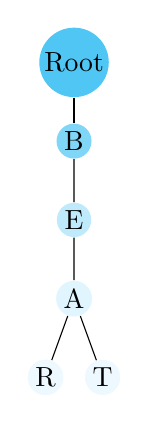
\begin{tikzpicture}
    [
    level distance=10mm,
    every node/.style={fill=cyan!69,circle,inner sep=1pt},
    level 1/.style={sibling distance=50mm,nodes={fill=cyan!50}},
    level 2/.style={sibling distance=25mm,nodes={fill=cyan!25}},
    level 3/.style={sibling distance=12.5mm,nodes={fill=cyan!12}},
    level 4/.style={sibling distance=7.25mm,nodes={fill=cyan!7}},
    ]
    \node {Root}
    child {node {B}
      child {node {E}
        child {node {A}
          child {node {R} }
          child {node {T} }
        }
      }
    };
  \end{tikzpicture}
  \\
  The longest common prefix in this Trie is "BEA".
\end{center}

Trie is used in operations like auto-completion and spell check.
Instead of comparing the misspelled word to every words in the spell check dictionary, Trie only requires a few traversals of the nodes.
In many spell checking algorithms, after morphological processing to handle grammatical variations, hash table is first used to check if a word exists in the dictionary.
Then, the word is searched in the Trie, and possible candidates are sorted based on the frequency in the language and Levenshtein distance.

\section{PATRICIA}

PATRICIA, or radix tree is a version of Trie where node can store words and not just characters.

\begin{center}
  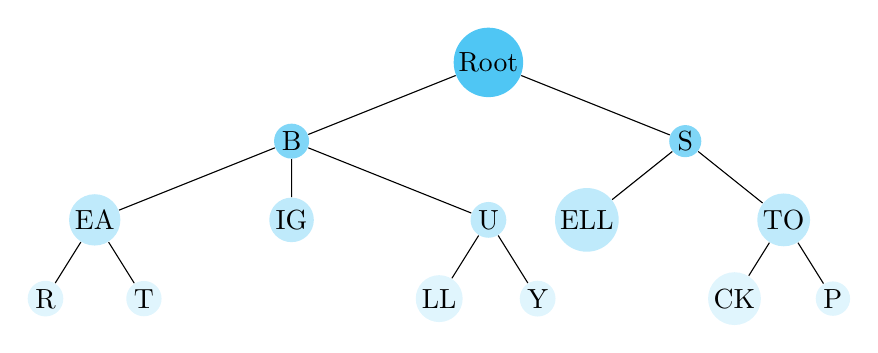
\begin{tikzpicture}
    [
    level distance=10mm,
    every node/.style={fill=cyan!69,circle,inner sep=1pt},
    level 1/.style={sibling distance=50mm,nodes={fill=cyan!50}},
    level 2/.style={sibling distance=25mm,nodes={fill=cyan!25}},
    level 3/.style={sibling distance=12.5mm,nodes={fill=cyan!12}},
    level 4/.style={sibling distance=7.25mm,nodes={fill=cyan!7}},
    level 5/.style={sibling distance=3.625mm,nodes={fill=cyan!3}},
    ]
    \node {Root}
    child {node {B}
      child {node {EA}
        child {node {R} }
        child {node {T} }
      }
      child {node {IG} }
      child {node {U}
        child {node {LL} }
        child {node {Y} }
      }
    }
    child {node {S}
      child {node {ELL} }
      child {node {TO}
          child {node {CK} }
          child {node {P} }
      }
    };
  \end{tikzpicture}
  \\
  PATRICIA with the following words: { BEAR, BEAT, BIG, BULL, BUY, SELL, STOCK, STOP }
\end{center}

\section{Huffman Coding}

Huffman Coding is a technique for lossless data compression.
The algorithm uses a specialized binary tree called Huffman tree to assign shorter ``prefix code'' more frequently used characters.

\noindent Supposed you have a data with the following frequency:
\begin{center}
  \begin{tabular}{ |c||c|c|c|c|c|c| }
    \hline
    Char & E & D & C & O & A & G\\
    \hline
    Frequency & 17 & 10 & 5 & 3 & 15 & 6\\
    \hline
  \end{tabular}
\end{center}

\noindent First, pick two nodes with the lowest frequencies and merge them into a binary tree, with the root note indicating the sum of the frequency.
When forming a subtree, assign $0$ to the edge to left node and $1$ to the edge to the right node.
Push the root back into the priority queue, pick two nodes or subtrees with the lowest frequencies, and merge them into a tree.
Repeat this process.

\begin{center}
  \begin{enumerate}
    \item Initially, $Q = \{ (O, 3), (C, 5), (G, 6), (D, 10), (A, 15), (E, 17) \}$.\\
      Merging O and C:\\
      \begin{forest}
        for tree={circle,draw, l sep=20pt}
        [8,blue
          [O,edge label={node[midway,left] {0} } ]
          [C,edge label={node[midway,right] {1} } ]
        ]
      \end{forest}
    \item $Q = \{ (G, 6), (\text{Subtree with (O, C): }, 8) (D, 10), (A, 15), (E, 17) \}$.\\
      Merging G and the subtree with O, C:\\
      \begin{forest}
        for tree={circle,draw, l sep=20pt}
        [14,blue
          [G,edge label={node[midway,left] {0} } ]
          [8,blue,edge label={node[midway,right] {1} }
            [O,edge label={node[midway,left] {0} } ]
            [C,edge label={node[midway,right] {1} } ]
          ]
        ]
      \end{forest}
    \item $Q = \{ (D, 10), (\text{Subtree with (O, C, G)}, 14), (A, 15), (E, 17) \}$.\\
      Merging D and the subtree with O, C, G:\\
      \begin{forest}
        for tree={circle,draw, l sep=20pt}
        [24,blue
          [D,edge label={node[midway,left] {0} } ]
          [14,blue,edge label={node[midway,right] {1} }
            [G,edge label={node[midway,left] {0} } ]
            [8,blue,edge label={node[midway,right] {1} }
              [O,edge label={node[midway,left] {0} } ]
              [C,edge label={node[midway,right] {1} } ]
            ]
          ]
        ]
      \end{forest}
    \item $Q = \{ (A, 15), (E, 17), (\text{Subtree with (O, C, G, D)}, 24) \}$.\\
      Merging A and E:\\
      \begin{forest}
        for tree={circle,draw, l sep=20pt}
        [32,blue
          [A,edge label={node[midway,left] {0} } ]
          [E,edge label={node[midway,right] {1} } ]
        ]
      \end{forest}
    \item $Q = \{ (\text{Subtree with (O, C, G, D)}, 24) (\text{Subtree with (A, E)}, 32) \}$.\\
      Merging two subtrees:\\
      \begin{forest}
        for tree={circle,draw, l sep=20pt}
        [56,blue
          % subtree 1
          [24,blue,edge label={node[midway,left] {0} }
            [D,edge label={node[midway,left] {0} } ]
            [14,blue,edge label={node[midway,right] {1} }
              [G,edge label={node[midway,left] {0} } ]
              [8,blue,edge label={node[midway,right] {1} }
                [O,edge label={node[midway,left] {0} } ]
                [C,edge label={node[midway,right] {1} } ]
              ]
            ]
          ]
          % subtree 2
          [32,blue,edge label={node[midway,right] {1} }
            [A,edge label={node[midway,left] {0} } ]
            [E,edge label={node[midway,right] {1} } ]
          ]
        ]
      \end{forest}
  \end{enumerate}
\end{center}

\noindent To determine the prefix code for each character, follow the 0's and 1's assigned to the edge.

\begin{center}
  \begin{tabular}{ |c||c|c|c|c|c|c| }
    \hline
    Char & E & D & C & O & A & G\\
    \hline
    Prefix Code & 11 & 00 & 0111 & 0110 & 10 & 010\\
    \hline
  \end{tabular}
\end{center}

\noindent To encode a string, say ``GOOD'' simply replace the characters with prefix code: ``010 0110 0110 00'' (spaces are added for the readability).

Here is the implementation in Python:

\begin{minted}{python}
import heapq
from collections import Counter


class HuffNode:
    def __init__(self, character=None, frequency=0):
        self.character = character
        self.frequency = frequency
        self.left = None
        self.right = None

    def __gt__(self, other):
        return self.frequency > other.frequency

    def __str__(self):
        return f"{self.character}: {self.frequency}"


def buildHuffmanTree(freq: dict):
    """
    Given the dictionary of frequency of each character, build a Huffman Tree
    :return: dict of character to respective code generated by Huffman coding
    """
    min_heap = [HuffNode(char, f) for char, f in freq.items()]
    heapq.heapify(min_heap)

    while len(min_heap) > 1:
        left = heapq.heappop(min_heap)
        right = heapq.heappop(min_heap)

        mergedSubtree = HuffNode(frequency=left.frequency + right.frequency)
        mergedSubtree.left = left
        mergedSubtree.right = right

        heapq.heappush(min_heap, mergedSubtree)

    return min_heap[0]  # root


def getCodeMap(root: HuffNode):
    """
    Given the root of the Huffman Tree, create a dictionary mapping
    character to the respective code generated by the tree.
    Left nodes get 0, right nodes get 1.
    :param root: root of the Huffman Tree, generated by buildHuffmanTree()
    :return: dict of character to respective code generated by Huffman coding
    """
    codeMap = {}

    def preorder(node, code=""):
        if node is None:
            return

        if node.character is not None:
            codeMap[node.character] = code
        preorder(node.left, code=code + '0')
        preorder(node.right, code=code + '1')

    preorder(root)
    return codeMap


def encode(pattern, codeMap):
    """
    Given a string and a Huffman dictionary, encode the string
    :param pattern: String to code
    :param codeMap: dict mapping character to code, generated by getCodeMap()
    :return: coded string
    """
    return "".join([codeMap[c] for c in pattern])



strr = "EEEEEEEEEEEEEEEEEDDDDDDDDDDCCCCCOOOAAAAAAAAAAAAAAAGGGGGG"
root = buildHuffmanTree(Counter(strr))
print(encode("GOOD", getCodeMap(root)))
\end{minted}

\noindent [Bonus] To decode a Huffman string, we can traverse the Huffman tree until we encounter a leaf node.

\begin{minted}{python}
def decode(pattern, root):
    """
    Given Huffman string and a Huffman tree, decode the string
    :param pattern: Huffman string to decode
    :param root: Root of the respective Huffman tree
    :return: decoded string
    """
    n = len(pattern)

    curr = root
    res = ""
    for i in range(n):
        if pattern[i] == '0':
            curr = curr.left
        else:
            curr = curr.right

        # Reached a leaf node
        # 1. if curr.character is not None
        # 2. if curr.frequency is None
        # 3. if curr.left is None and curr.right is None
        # above three are all logically same in this context,
        # as nodes in Huffman tree contains either frequency or character
        # and leaf nodes are always the ones that contain the character
        if curr.character is not None:
            res += curr.character
            curr = root  # reset to the root

    return res


root = buildHuffmanTree({"E": 17, "D": 10, "C": 5, "O": 3, "A": 15, "G": 6})
print(decode("000110010", root))
# ...
"DOG"  # !!
\end{minted}

